\documentclass{article}
\usepackage[letterpaper, landscape, left=0.5in, right=0.5in, top=2.25in, bottom=2.25in]{geometry}

\usepackage{showframe}
\usepackage{tikz}
\usepackage[default]{sourcesanspro}
\usepackage[T1]{fontenc}
\pagenumbering{gobble}

\newenvironment{sentencediagram}[5]
    {
        \newgeometry{top=#1in, bottom=#1in, left=#2in, right=#2in}
        \vspace*{\fill}
        \begin{center}
            {
                \fontfamily{cmr}\selectfont
                #3
            }

            \vspace{0.4cm}
            \footnotesize #4, \textit{#5} \\
            \vspace{0.5cm}
            \Large 
    }
    {
        \end{center}
        \vspace*{\fill}
        \clearpage
        \restoregeometry
    }

\tikzstyle{every path}=[line width=1.6pt]
\tikzstyle{every node} = [above=-0.15cm]

\definecolor{subjectnoun}{RGB}{106,120,132}
\definecolor{copula}{RGB}{124,139,111}
\definecolor{subjectcomplement}{RGB}{95,61,26}
\definecolor{conjunction}{RGB}{45,75,120}
\definecolor{preposition}{RGB}{81,167,204}
\definecolor{directobject}{RGB}{252,87,156}
\definecolor{adjective}{RGB}{103,81,120}
\definecolor{noun}{RGB}{180,78,60}
\definecolor{predicateverb}{RGB}{176,161,118}
\definecolor{article}{RGB}{92,133,42}
\definecolor{pronoun}{RGB}{163,120,198}
\definecolor{adverb}{RGB}{133,188,114}
\definecolor{modalverb}{RGB}{230,60,92}
\definecolor{infinitiveverb}{RGB}{101,154,148}
\definecolor{verb}{RGB}{226,160,80}

\usetikzlibrary{positioning}

\begin{document}
    \Large 
    \vspace*{\fill}
    \begin{center}
        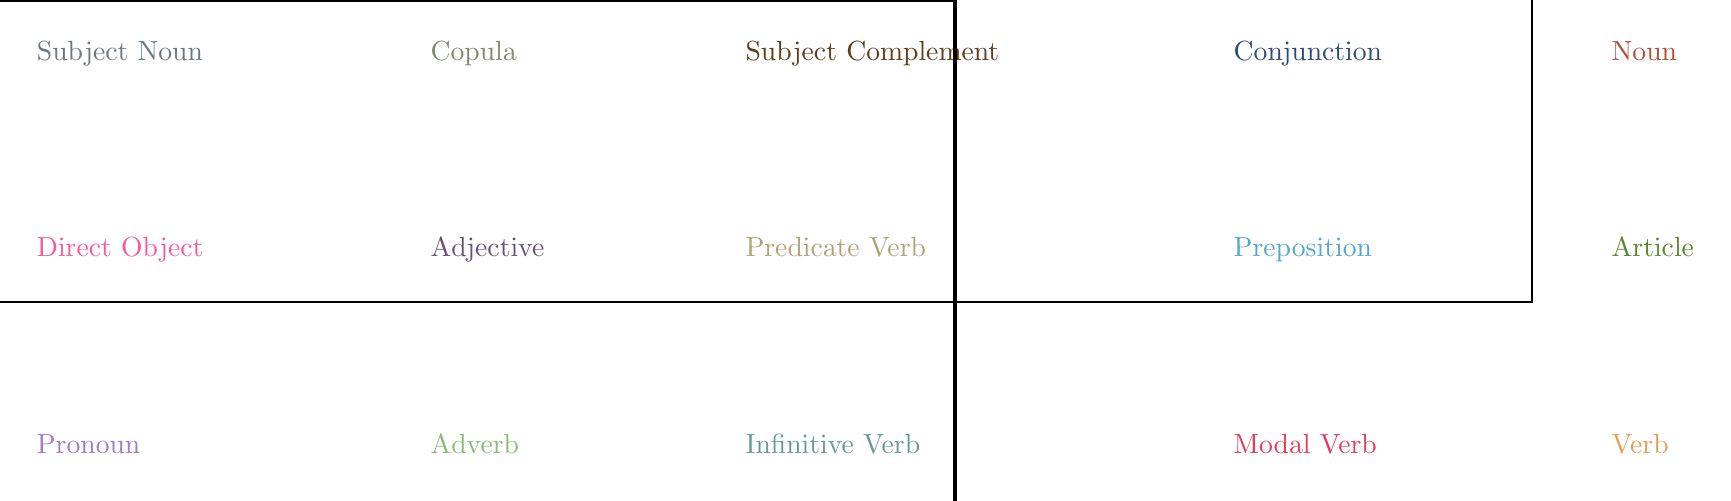
\begin{tikzpicture}
            \node[text=subjectnoun, anchor=west] at (-11, 2.5) {\strut Subject Noun};
            \node[text=copula, anchor=west] at (-6, 2.5) {\strut Copula};
            \node[text=subjectcomplement, anchor=west] at (-2, 2.5) {\strut Subject Complement};
            \node[text=conjunction, anchor=west] at (4.2, 2.5) {\strut Conjunction};
            \node[text=noun, anchor=west] at (9, 2.5) {\strut Noun};
            \node[text=directobject, anchor=west] at (-11, 0) {\strut Direct Object};
            \node[text=adjective, anchor=west] at (-6, 0) {\strut Adjective};
            \node[text=predicateverb, anchor=west] at (-2, 0) {\strut Predicate Verb};
            \node[text=preposition, anchor=west] at (4.2, 0) {\strut Preposition};
            \node[text=article, anchor=west] at (9, 0) {\strut Article};
            \node[text=pronoun, anchor=west] at (-11, -2.5) {\strut Pronoun};
            \node[text=adverb, anchor=west] at (-6, -2.5) {\strut Adverb};
            \node[text=infinitiveverb, anchor=west] at (-2, -2.5) {\strut Infinitive Verb};
            \node[text=modalverb, anchor=west] at (4.2, -2.5) {\strut Modal Verb};
            \node[text=verb, anchor=west] at (9, -2.5) {\strut Verb};
        \end{tikzpicture}
    \end{center}
    \vspace*{\fill}
\end{document}
